%STILL NEEDS FINISHING
%haven't solved yet, certainly too hard for AS. NOW SOLVED 4/12/13 
\begin{problem} [A1988FMIIQ1a] %friction, balancing forces
%diagram removed, some points not named %I changed this quite a lot - there were problems with the original diagram not being entirely free body which meant scrappy minus signs resulting in a negative coefficient of friction. Hopefully now correct. JZ
{\exposition{Two rough uniform spheres A and B have radii \vari{8a} and \vari{4a} and masses \vari{4m} and \vari{m} respectively. The spheres rest on a rough horizontal table in contact with one another at a point C. A horizontal force of magnitude \vari{2mg} is applied to the highest point on A, D. The line of action of this force and all the points mentioned lie in the same vertical plane.}

\begin{enumerate}
	\item \question[a]{Show that the magnitude of the frictional force at the base of A is zero.}
	\item \question[b]{For \valuedef{m}{0.5}{kg}, find the magnitude of the normal reaction at the base of A.}
	\item \question[c]{The coefficient of friction between the two spheres and between each sphere and the table is \vari{\mu}. Find the smallest value of \vari{\mu} for which the balls remain at equilibrium.}
\end{enumerate}}
{\textit{Adapted with permission from UCLES, A Level Further Maths, Syllabus C, June 1988, Paper II, Question 1}}
{\answer[a]{}
\answer[b]{\valuedef{N_A}{mg(4-2\sqrt 2)}{.} Substituting in \valuedef{m}{5}{kg} gives \valuedef{N_A}{5.75}{kg}}
\answer[c]{\valuedef{\mu}{\frac{1}{\sqrt{2}}}}
Diagrams \ref{fig:Statics_twospheres} and \ref{fig:Statics_twospheresforces} show the geometry and the forces acting on the spheres respectively:
\begin{figure}[h]
\centering
\begin{subfigure}{0.5\textwidth}
\centering
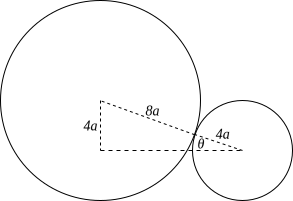
\includegraphics[width=0.95\linewidth]{Statics_twospheres}
\caption{}
\label{fig:Statics_twospheres}
\end{subfigure}%
\begin{subfigure}{0.5\textwidth}
\centering
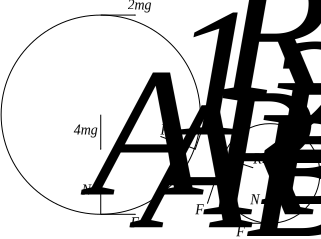
\includegraphics[width=0.95\linewidth]{Statics_twospheresforces}
\caption{}
\label{fig:Statics_twospheresforces}
\end{subfigure}
\caption{}
\end{figure}
\\
\begin{enumerate}
\item
There are several ways to find the forces in this question, and each will involve resolving forces and taking moments about different points. For the first part, I took moments about the centre of each sphere and resolved the forces acting on each into horizontal components. First, the horizontal forces on A:
\begin{align}
2mg+F\s A+F\s R \sin\theta=R_1\cos\theta \label{eq:Statics_twospheres1}
\end{align}
and the moments about the centre of $A$
\begin{align}
2mg(8a)&=F\s A(8a)+F\s R(8a) \notag \\
\Rightarrow 2mg&=F\s A +F\s R \label{eq:Statics_twospheres2}
\end{align}
Then the horizontal forces on $B$
\begin{align}
R_2\cos\theta=F\s R\sin\theta+F\s B \label{eq:Statics_twospheres3}
\end{align}
and finally the moments about the centre of B
\begin{align}
F\s R(4a)-F\s B(4a)&=0 \notag \\
\Rightarrow F\s R&=F\s B \label{eq:Statics_twospheres4}
\end{align}
This gives us the required four equations to solve for the four unknowns, $F\s A, F\s B, F\s R$ and $R$. Using the result from \eqref{eq:Statics_twospheres4} in \eqref{eq:Statics_twospheres3} we find
\begin{align}
R_2\cos\theta=F\s R\sin\theta&+F\s R \notag \\
\Rightarrow R_2&=\frac{1+\sin\theta}{\cos\theta}F\s R \label{eq:Statics_twospheres5}
\end{align}
and then using that result, an expression for $F\s R$ from \eqref{eq:Statics_twospheres2} and Newton's 3rd law to deduce $R_2=R_1$ we find:
\begin{align*}
2mg+F\s A+(2mg-F\s A)\sin\theta&=\frac{1+\sin\theta}{\cos\theta}(2mg-F\s A)\cos\theta \\ 
\Rightarrow 2mg+F\s A&=(2mg-F\s A)(1+\sin\theta-\sin\theta) \\
\Rightarrow 2mg+F\s A&=2mg-F\s A \\
\Rightarrow F\s A&=0
\end{align*}
\item
We need an additional equation involving $N\s A$, and we can resolve vertically on $A$ to obtain it:
\begin{align*}
N\s A+R_1\sin\theta+F\s R\cos\theta=4mg
\end{align*}
Use the previous equations to substitute in expressions for $R_1$ and $F\s R=2mg$:
\begin{align*}
N\s A&=4mg-\frac{1+\sin\theta}{\cos\theta}2mg\sin\theta-2mg\cos\theta \\
\Rightarrow N\s A&=mg\left(4-2(1+\sin\theta)\tan\theta-2\cos\theta\right) 
\end{align*}
From diagram \ref{fig:Statics_twospheres} we can see that 
\begin{align*}
\sin\theta=\frac{4a}{8a+4a}&=\frac{1}{3} \\
\Rightarrow \cos\theta&=\sqrt{1-\frac{1}{9}}=\frac{2\sqrt 2}{3} \\
\Rightarrow \tan\theta&=\frac{\sqrt{2}}{4} 
\end{align*}
So finally we get
\begin{align*}
N\s A&=mg\left(4-2\left(1+\frac{1}{3}\right)\frac{\sqrt{2}}{4}-2\frac{2\sqrt 2}{3}\right) \\
&=mg\left(4-\frac{4}{3}2\sqrt 2-\frac{2}{3}2\sqrt 2\right) \\
\Rightarrow N\s A&=mg(4-2\sqrt 2)
\end{align*}

Substituting in $m$ = 5~kg gives $N_A$ = 5.75~kg
\item
At the point where the two spheres touch, we have
\begin{align*}
 F\s R&\le \mu R_1 \\
\Rightarrow \mu&\ge\frac{F\s R}{R_1}=\frac{\cos\theta}{1+\sin\theta} \\
\Rightarrow \mu&\ge\frac{1}{\sqrt 2}
\end{align*}
where the last step follows from equation \eqref{eq:Statics_twospheres5}. We also have another condition from the bottom of $B$:
\begin{align*}
F\s B&\le\mu N\s B \\
\Rightarrow \mu&\ge\frac{F\s B}{N\s B}
\end{align*}
We now need to resolve vertically on $B$ to find an expression for $N\s B$ (we already have, from equation \eqref{eq:Statics_twospheres4}, that $F\s B=F\s R=2mg$):
\begin{align*}
N\s B=F\s R\cos\theta&+R_2\sin\theta+mg \\
\Rightarrow N\s B&=mg+F\s R\left(\cos\theta+\frac{1+\sin\theta}{\cos\theta}\sin\theta\right) \\
\Rightarrow N\s B&=mg+2mg\left(\frac{2\sqrt 2}{3}+\frac{4}{3}\frac{1}{2\sqrt 2}\right) \\
\Rightarrow N\s B&=mg(1+2\sqrt 2)
\end{align*}
Finally we have:
\begin{align*}
\mu\ge\frac{2}{1+2\sqrt{2}} \\
\\ \mu \ge \frac{4\sqrt{2}-2}{7}
\end{align*}
Since 
\begin{align*}
\frac{1}{\sqrt{2}} > \frac{4\sqrt{2}-2}{7}
\end{align*}
The smallest value of \vari{\mu} we can have for equilibrium is:
\begin{align*}
\mu = \frac{1}{\sqrt{2}}
\end{align*}

\end{enumerate}
}
\end{problem}